%%%%%%%%%%%%%%%%%%%%%%%%%%%%%%%%%%%%%%%%%%%%%%%%%%%%%%%%%%%%%%%
%
% Welcome to Overleaf --- just edit your LaTeX on the left,
% and we'll compile it for you on the right. If you open the
% 'Share' menu, you can invite other users to edit at the same
% time. See www.overleaf.com/learn for more info. Enjoy!
%
%%%%%%%%%%%%%%%%%%%%%%%%%%%%%%%%%%%%%%%%%%%%%%%%%%%%%%%%%%%%%%%
\documentclass[12pt, letterpaper]{article}
\usepackage{graphicx}
\usepackage[T1]{fontenc}
\usepackage[utf8]{inputenc}
\usepackage{amsmath}
\usepackage{float}
\usepackage{booktabs}
\usepackage{tikz}
\usetikzlibrary{positioning}
\usetikzlibrary{arrows.meta, decorations.markings}
\usetikzlibrary{calc}
\usepackage{xcolor}
\usepackage{listings}
\usepackage{parskip} 
\lstdefinestyle{octave}{
    language=Octave,
    basicstyle=\ttfamily\small,
    keywordstyle=\color{blue}\bfseries,
    commentstyle=\color{gray}\itshape,
    stringstyle=\color{teal},
    numbers=left,
    numberstyle=\tiny\color{gray},
    stepnumber=1,
    numbersep=8pt,
    frame=single,
    rulecolor=\color{black!30},
    breaklines=true,
    tabsize=4,
    showstringspaces=false,
    literate={č}{{\v{c}}}1 {ć}{{\'{c}}}1 {ž}{{\v{z}}}1 {š}{{\v{s}}}1 {đ}{{\dj{}}}1
             {Č}{{\v{C}}}1 {Ć}{{\'{C}}}1 {Ž}{{\v{Z}}}1 {Š}{{\v{S}}}1 {Đ}{{\DJ{}}}1
}
% Makes figures numbered as <section>.<figure> (e.g., Slika 1.1)
\numberwithin{figure}{section}
\graphicspath{{images/}}
\title{Primjene mjere sličnosti grafova}
\author{Vid Joha}
\date{Studeni 2026.}
\begin{document}
\maketitle
\begin{abstract}
Primjenom metode mjerenja sličnosti 2 grafa ću usporediti koliko su njihovi određeni vrhovi slični, to jest različiti. Sličnost 2 grafa ću odrediti pomoću matrice sličnosti koju ću dobiti višestrukom iteracijom sljedeće formule.\[X_{k+1} = BX_kA^T + B^TX_kA\] gdje su A i B matrice susjedstava grafova $G_A$ i $G_B$, a $X_k$ je neka matrica sa pozitivnim elementima.
Različitim brojem iteracija možemo saznati koliko i na koji način su 2 grafa slična.
\end{abstract}

\section{Uvod}
Razne stvari poput prijateljskih odnosa, navika kupovanja, riječi u dokumentu ili molekula možemo prikazati u obliku grafova. Vrhovi tih grafova su tada ljudi, stvari ili atomi, a bridovi su veze između njih. Takav graf ćemo označiti sa $G_A$ gdje je $A$ pripadna matrica susjedstava. Takva matrica je dimenzija $n\times{n}$ gdje je $n$ broj vrhova grafa $G_A$. Element $A[i][j]$ te matrice će biti $1$ ako postoji brid iz vrha $i$ u vrh $j$, a $0$ ako takav brid ne postoji. Očigledno će takve matrice biti simetrične za neusmjerene grafove. 

\begin{figure}[H]
    \centering
    % Left side: TikZ Graph
    \begin{minipage}[c]{0.48\textwidth}
        \centering
        \begin{tikzpicture}[
            scale=0.65, transform shape,
            decoration = {markings,
                          mark=at position .5 with {\arrow{Stealth[length=2mm]}}},
            dot/.style = {circle, fill, inner sep=2.4pt, node contents={},
                          label=#1},
            every edge/.style = {draw, postaction=decorate}
        ]
            \node (a) at (0,5) [dot=$a$];
            \node (b) at (1,2) [dot=below:$b$];
            \node (c) at (4,2) [dot=$c$];
            \node (d) at (6,4) [dot=right:$d$];
            \node (e) at (3,0) [dot=right:$e$];

            \path (a) edge (b)
                  (b) edge (c)
                  (c) edge (d)
                  (c) edge (e)
                  (d) edge[bend left] (c);
        \end{tikzpicture}
    \end{minipage}% <--- Keep this % sign (no blank line between minipages!)
    \hfill
    % Right side: Adjacency Matrix
    \begin{minipage}[c]{0.48\textwidth}
        \[
        A = \begin{pmatrix}
        0 & 1 & 0 & 0 & 0 \\
        0 & 0 & 1 & 0 & 0 \\
        0 & 0 & 0 & 1 & 1 \\
        0 & 0 & 1 & 0 & 0 \\
        0 & 0 & 0 & 0 & 0
        \end{pmatrix}
        \]
    \end{minipage}
    \caption{Usmjereni graf $G_A$ i pripadna matrica susjedstava $A$.}
    \label{fig:graf_matrica}
\end{figure}

\section{Teorija}
 J. M. Kleinberg u svojoj knjizi Authoritative sources in a hyperlinked environment ~\cite{kleinberg1999} predstavlja metodu za pronalazak najboljih stranica na internetu. Metoda se bazira na hubovima i autoritetima. Stranica je dobar hub ako vodi do dobrih autoriteta, a dobar je autoritet ako do nje vode dobri hubovi. Ocjene za to koliko je stranica dobar hub ili autoritet se mogu dobiti iterativnim procesom:
 \begin{enumerate}
  \item Ocjene hubova i autoriteta počnu kao nasumične pozitivne vrijednosti.
  \item Nove hub i autoritet ocjene se računaju na sljedeći način:
  \[
\begin{cases}
h_j \leftarrow \sum_{i:(j,i)\in E} a_i, \\
a_j \leftarrow \sum_{i:(i,j)\in E} h_i.
\end{cases}
\]
\end{enumerate}
Hub ocjena vrha $j$ je jednaka sumi autoritet ocjena vrhova na koje vrh $j$ pokazuje, a autoritet ocjena vrha $j$ je jednaka sumi hub ocjena vrhova koji pokazuju na $j$. Ako sa B označimo matricu čiji je element B[i][j] jednak broju vrhova između vrhova $i$ i $j$ (matrica susjedstava grafa), tada se gornja jednadžba može zapisati u kompaktnom matričnom obliku.
\[
\begin{bmatrix}
h \\
a
\end{bmatrix}_{k+1}
=
\begin{bmatrix}
0 & B \\
B^T & 0
\end{bmatrix}
\begin{bmatrix}
h \\
a
\end{bmatrix}_{k},
\quad k = 0, 1, \dots,
\]
Nadalje ako zapišemo gornje matrice kao 
\[
x_k = \begin{bmatrix}
h \\
a
\end{bmatrix}_{k},
\quad
M = \begin{bmatrix}
0 & B \\
B^T & 0
\end{bmatrix}.
\]
gornja jednadžba se može skratiti na sljedeći zapis.
\[
x_{k+1} = M x_k, \quad k = 0, 1, \dots,
\]
Zanimaju nas samo relativne ocjene tako da ćemo ih normalizirati. $\|\cdot\|_2$ je euklidska norma.
\begin{equation}
z_0 = x_0 > 0, \quad z_{k+1} = \frac{M z_k}{\|M z_k\|_2}, \quad k = 0, 1, \dots,
\end{equation}
Niz $z_k$ generalno ne konvergira nego oscilira između dvije vrijednosti
\[
z_{\text{even}} = \lim_{k\to\infty} z_{2k} \quad \text{and} \quad z_{\text{odd}} = \lim_{k\to\infty} z_{2k+1}.
\]
Sada poopćujemo ovu konstrukciju. Ocjena autoriteta vrha $j$ grafa $G$ može se shvatiti kao ocjena sličnosti između vrha $j$ grafa $G$ i vrha $\mathit{authority}$ grafa
\[
\mathit{hub} \longrightarrow \mathit{authority}
\]

i, slično tome, ocjena huba vrha $j$ grafa $G$ može se promatrati kao ocjena sličnosti između vrha $j$ i vrha $\mathit{hub}$. Iteracija međusobnog pojačavanja i ažuriranja koja je gore korištena može se poopćiti i na grafove koji se razlikuju od strukturnog grafa $\mathit{hub}\text{--}\mathit{authority}$. Ideju ovog poopćenja ilustriramo na primjeru. 
Neka su grafovi G i S

\hspace{2cm}
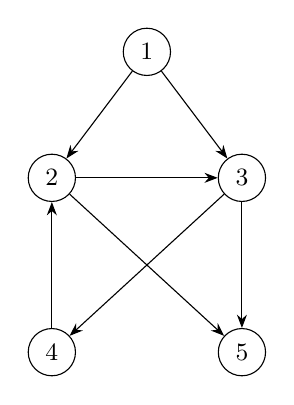
\begin{tikzpicture}[
    >=Stealth,
    node distance=1.6cm and 1.8cm,
    vertex/.style={circle, draw, minimum size=6mm, inner sep=0pt, font=\small}
]
    \node[vertex] (v2) {2};
    \node[vertex, right=of v2] (v3) {3};
    \node[vertex] (v1) at ($(v2)!0.5!(v3) + (0,1.6cm)$) {1};
    \node[vertex, below=of v2] (v4) {4};
    \node[vertex, below=of v3] (v5) {5};

    \draw[->] (v1) -- (v2);
    \draw[->] (v1) -- (v3);

    \draw[->] (v2) -- (v3);
    \draw[->] (v3) -- (v4);

    \draw[->] (v2) -- (v5);
    \draw[->] (v3) -- (v5);
    \draw[->] (v4) -- (v2);
\end{tikzpicture}
\hspace{2cm}
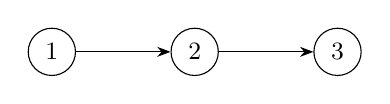
\begin{tikzpicture}[
    >=Stealth,
    node distance=1.6cm and 1.2cm,
    vertex/.style={circle, draw, minimum size=6mm, inner sep=0pt, font=\small}
]
    \node[vertex] (v1) {1};
    \node[vertex, right=of v1] (v2) {2};
    \node[vertex, right=of v2] (v3) {3};

    \draw[->] (v1) -- (v2);
    \draw[->] (v2) -- (v3);
\end{tikzpicture}

Njihove matrice susjedstava su
\[
G =
\begin{bmatrix}
0 & 1 & 1 & 0 & 0 \\
0 & 0 & 1 & 0 & 1 \\
0 & 0 & 0 & 1 & 1 \\
0 & 1 & 0 & 0 & 0 \\
0 & 0 & 0 & 0 & 0
\end{bmatrix},
\qquad
S =
\begin{bmatrix}
0 & 1 & 0 \\
0 & 0 & 1 \\
0 & 0 & 0
\end{bmatrix}
\]
Svakom vrhu $j$ grafa $G$ sada pridružujemo tri ocjene $x_{i1}, x_{i2}$ i $x_{i3}$, po jednu za svaki vrh grafa S. Te ocjene inicijaliziramo nekom pozitivnom vrijednošću i zatim ih iteriramo prema sljedećoj relaciji međusobnog pojačavanja:
\[
\begin{cases}
x_{i1} \leftarrow \sum_{j:(i,j)\in E} x_{i2}, \\
x_{i2} \leftarrow \sum_{j:(j,i)\in E} x_{i1} & + \sum_{j:(i,j)\in E} x_{i3}, \\
x_{i3} \leftarrow \sum_{j:(j,i)\in E} x_{i2},
\end{cases}
\]

\begin{lstlisting}[style=octave, caption={Implementacija algoritma u Octaveu}, label={lst:blondel}]
1;

function Z = blondel_slicnost(A, B, Z0, maxIter, tol)
  Z = Z0 / norm(Z0, 'fro');
    for it = 1:maxIter
        Zold = Z;
        for step = 1:2
            Z = B*Z*A' + B'*Z*A;
            Z = Z / norm(Z, 'fro');
        end
        if norm(Z - Zold, 'fro') < tol
            break;
        end
    end
end

maxIter   = 100;
tol       = 1e-9;

matrica_Susjedstava_G = [0,1,1,0,0;
                      0,0,1,0,1;
                      0,0,0,1,1;
                      0,1,0,0,0;
                      0,0,0,0,0]

matrica_Susjedstava_S = [0,1,0;
                        0,0,1;
                        0,0,0]

Z0 = ones(size(matrica_Susjedstava_G,1),size(matrica_Susjedstava_S,1))

Z = blondel(matrica_Susjedstava_S,matrica_Susjedstava_G,Z0,maxIter,tol);

Z
\end{lstlisting}
Matrica sličnosti grafova G i S je
\[
Z =
\begin{bmatrix}
0.4433 & 0.1043 & 0 \\
0.2801 & 0.3956 & 0.0858 \\
0.0858 & 0.3956 & 0.2801 \\
0.2216 & 0.0489 & 0.2216 \\
0 & 0.1043 & 0.4433
\end{bmatrix}
\]
Vrh 1 iz grafa G je najsličniji vrhu 1 iz grafa S.\\
Vrhovi 2 i 3 su najsličniji vrhu 2 iz grafa S.\\
Vrh 5 je najsličniji vrhu 3 iz grafa S.

Sada dolazimo do opisa općeg slučaja. Pretpostavimo da imamo dva usmjerena grafa $G_A$ i $G_B$ s $n_A$ i $n_B$ vrhova te skupovima bridova $E_A$ i $E_B$. Graf $G_A$ promatramo kao strukturni graf koji ima ulogu grafova $\mathit{hub} \longrightarrow \mathit{authority}$ i $1 \longrightarrow 2 \longrightarrow 3$ u gornjim primjerima. Promatramo realne ocjene $x_{ij}$ za $i = 1, \dots, n_B$ i $j = 1, \dots, n_A$ te istodobno ažuriramo sve ocjene prema sljedećim jednadžbama ažuriranja:
\[
x_{ij} \leftarrow \sum_{r:(r,i)\in E_B,\; s:(s,j)\in E_A} x_{rs} + \sum_{r:(i,r)\in E_B,\; s:(j,s)\in E_A} x_{rs}.
\]


Ova jednadžba se može interpretirati kao produktni graf od $G_A$ i $G_B$. \emph{Produktni graf} od $G_A$ i $G_B$ je graf koji ima $n_A \cdot n_B$ vrhova i koji ima brid između vrhova $(i_1, j_1)$ i $(i_2, j_2)$ ako postoji brid između $i_1$ i $i_2$ u $G_A$ te postoji brid između $j_1$ i $j_2$ u $G_B$. Gornja jednadžba ažuriranja tada je ekvivalentna zamjeni ocjena svih vrhova produktnog grafa sumom ocjena vrhova povezanih izlaznim ili ulaznim bridom.

Jednadžba se može zapisati i u kompaktnijem matričnom obliku. Neka je $Z_k$ matrica dimenzija $n_B \times n_A$ s članovima $x_{ij}$ u iteraciji $k$. Tada jednadžbe ažuriranja poprimaju jednostavan oblik
\begin{equation}
Z_{k+1} = B Z_k A^T + B^T Z_k A, \quad k = 0, 1, \dots,
\end{equation}

gdje su $A$ i $B$ matrice susjedstva grafova $G_A$ i $G_B$. U teoremu 2 i 3 dokazujemo da normirane parne i neparne iteracije ovog niza konvergiraju i da limes $Z_{even}(\mathbf{1})$ ima najveću normu od svih takvih limesa.

Ako prethodni niz normiramo dobivamo
\[
Z_{k+1} = \frac{B Z_k A^T + B^T Z_k A}{\|B Z_k A^T + B^T Z_k A\|_F}, \quad k = 0, 1, \dots.
\]
te sada možemo definirati S kao

\[
\mathbf{S} = \lim_{k \to +\infty} Z_{2k}
\]
Uzimamo matricu $\mathbf{S}$ kao definiciju matrice sličnosti između $G_A$ i $G_B$. Primijetimo da iz ove definicije slijedi da je matrica sličnosti između $G_B$ i $G_A$ transponirana matrica sličnosti između $G_A$ i $G_B$.

Izravan algoritamski zapis definicije dovodi do aproksimacijskog algoritma za računanje matrica sličnosti grafova:
\begin{enumerate}
    \item Postavimo $Z_0 = \mathbf{1}$.
    \item Iteriramo paran broj puta
    \[
    Z_{k+1} = \frac{B Z_k A^T + B^T Z_k A}{\|B Z_k A^T + B^T Z_k A\|_F}
    \]
    i zaustavljamo se pri konvergenciji.
    \item Izlaz $\mathbf{S}$ posljednja je vrijednost od $Z_k$.
\end{enumerate}
\section{Primjene}
\subsection{Gradovi Europe}

Prvi primjer je mala mreža zračnih letova između $33$ europska grada (od Amsterdama do Zagreba). Vrhovi grafa su gradovi, a brid između dva grada postoji ako među njima postoji direktan let. Graf je neusmjeren pa je matrica susjedstava simetrična. Matrica je spremljena u datoteci \texttt{matrica\_Gradova.txt} i dimenzija joj  $33\times 33$ s elementima $0$ i $1$. Gradovi su poredani abecedno, tako da je Zagreb posljednji vrh (indeks $n=33$). Zanima nas kojem je gradu Zagreb najsličniji. Rezultat metode iz seminara usporedit ćemo s kosinusnom sličnosti, koja gleda samo koliko dva grada imaju zajedničkih direktnih odredišta.

Funkcija \texttt{blondel\_slicnost} iz Listinga~\ref{lst:blondel} spremljena je u zasebnu datoteku \texttt{blondel\_slicnost.m}. Za usporedbu pišemo i pomoćnu funkciju koja računa kosinusnu sličnost redaka binarne matrice $B$:
\[
S_{ij} = \frac{\sum_k B_{ik}B_{jk}}{\sqrt{d_i\, d_j}},
\]
gdje je $d_i$ broj jedinica u retku $i$. Brojnik je broj zajedničkih susjeda vrhova $i$ i $j$.

\begin{lstlisting}[style=octave, caption={Pomoćna funkcija za kosinusnu sličnost}, label={lst:cos_gradovi}]
1;
function [S, common, d] = cosineSimilarity(B)
    N      = size(B, 1);
    d      = full(sum(B, 2));
    Bn     = spdiags(1 ./ sqrt(d), 0, N, N) * B;   % rows scaled to unit length
    S      = full(Bn * Bn');
    common = full(B * B');
end
\end{lstlisting}
Funkcija izračuna stupnjeve $d$, svaki redak podijeli njegovom duljinom $\sqrt{d_i}$ (matrica \texttt{Bn} ima retke jedinične duljine) i onda je \texttt{Bn*Bn'} upravo matrica kosinusa kuteva između redaka. Matrica \texttt{common} \,$= BB^T$ sadrži broj zajedničkih susjeda.

Sljedeći dio učitava matricu susjedstava i definira popis gradova, čiji redoslijed mora odgovarati redoslijedu redaka u datoteci.

\begin{lstlisting}[style=octave, caption={Učitavanje grafa direktnih letova}, label={lst:gradovi_ucitavanje}]
graf_Direktnih_letova = load('matrica_Gradova.txt');

cities = {
  'Amsterdam', 'Atena', 'Belgrade', 'Berlin', 'Bern', 'Bratislava', ...
  'Bruxelles', 'Budapest', 'Bucharest', 'Copenhagen', 'Dublin', ...
  'Helsinki', 'Istanbul', 'Lisabon', 'Ljubljana', 'London', ...
  'Luxemburg', 'Madrid', 'Minsk', 'Oslo', 'Paris', 'Prague', ...
  'Reykyavik', 'Riga', 'Rome', 'Sarajevo', 'Sofia', 'Stockholm', ...
  'Talin', 'Vienna', 'Vilnius', 'Warsaw', 'Zagreb'
};
maxIter   = 100;
tol       = 1e-9;
n = numel(cities);
\end{lstlisting}
graf\_Direktnih\_Letova sadrži gustu matricu u kojem je element [\textit{i}][\textit{j}] == 1 ako postoji direktni let između grada \textit{i} i grada \textit{j}. Parametri \texttt{maxIter} i \texttt{tol} određuju najveći broj dvostrukih koraka i prag konvergencije u funkciji \texttt{blondel\_slicnost}. Varijabla \texttt{n} je broj gradova, ali ujedno i indeks Zagreba.

Pošto računamo sličnost grafa sa samim sobom u funkciju blondel\_slicnost stavljamo $A=B$. Time dobivamo matricu $S$ čiji element $S_{ij}$ govori koliko je grad $i$ sličan gradu $j$. Početna matrica $Z_0$ je matrica jedinica, kao u algoritmu iz teorije.

\begin{lstlisting}[style=octave, caption={Iterativna metoda: najsličniji grad Zagrebu}, label={lst:gradovi_blondel}]
Z0 = ones(n, n);
S = blondel_slicnost(graf_Direktnih_letova, graf_Direktnih_letova, Z0, maxIter, tol);

s1 = S(n, :);              
s1(n) = -Inf;             
[val, ind] = max(s1);

fprintf('Najslicniji grad Zagrebu (iterativna metoda) je %s \n', cities{ind});
\end{lstlisting}
Redak \texttt{S(n,:)} sadrži ocjene sličnosti Zagreba sa svim gradovima. Budući da je graf uspoređen sam sa sobom, vrh je uvijek jako sličan samom sebi, pa se taj element isključuje. 

Sada isto radimo sa kosinusnom sličnosti.

\begin{lstlisting}[style=octave, caption={Kosinusna sličnost i spremanje rezultata}, label={lst:gradovi_cos}]
S2 = cosineSimilarity(graf_Direktnih_letova);
s2 = S2(n, :);
s2(n) = -Inf;              
[val2, ind2] = max(s2);
fprintf('Najslicniji grad Zagrebu (kosinus metoda) je %s\n', cities{ind2});
\end{lstlisting}
Kosinusna sličnost uspoređuje samo izravne susjede, to jest dva su grada slična ako imaju mnogo zajedničkih direktnih odredišta. Iterativna metoda dodatno uzima u obzir i susjede susjeda, i tako dalje, pa uspoređuje cjelokupnu strukturu mreže oko dva grada. Zato dvije metode ne moraju dati isti odgovor.

Pokretanjem porgrama dobivamo ispis:

Najslicniji grad Zagrebu (kosinus metoda) je London\\
Najslicniji grad Zagrebu (iterativna metoda) je Bucharest

\subsection{Wiki vote}

\textbf
Skup \emph{wiki-Vote} dolazi iz zbirke SNAP~\cite{leskovec2010}. Sadrži podatke o glasanju za izbor administratora na Wikipediji (do siječnja 2008.). Vrhovi grafa su korisnici Wikipedije ($7115$ vrhova), a usmjereni brid $i\to j$ znači da je korisnik $i$ glasao za korisnika $j$ kao kandidata za administratora. Graf ima $103689$ bridova. Datoteka \texttt{wiki-Vote.txt} je tekstualna lista parova \texttt{FromNodeId ToNodeId}. Zanima nas koji su glasači međusobno slični. Opet sličnost definiramo na dva načina: kosinusnom sličnosti, gdje su dva glasača slična ako su glasala o istim kandidatima, i iterativnom metodom, gdje su slični ako imaju sličnu ulogu u mreži glasanja.

Graf je prevelik za matricu $7115\times 7115 $ sličnosti u punom obliku, pa analizu ograničavamo na najaktivnije glasače. Prvi dio koda postavlja parametre.

\begin{lstlisting}[style=octave, caption={Parametri analize}, label={lst:wiki_parametri}]
clear; clc;

minimalan_Broj_Glasova  = 10;    
max_Broj_Glasaca      = 500;     
broj_Najslicnijih_Parova      = 10;      
max_Iteracija   = 100;     
granica_Konvergencije       = 1e-9;
\end{lstlisting}
Zadržavamo samo glasače koji su glasali barem \texttt{minimalan\_Broj\_Glasova} puta, a ako ih je više od \texttt{max\_Broj\_Glasaca}, uzimaju se najaktivniji. Preostali parametri određuju koliko se najsličnijih parova ispisuje te zaustavljanje iterativne metode. Funkcija \texttt{cosineSimilarity} je ista kao u Listingu~\ref{lst:cos_gradovi} i definirana je na početku skripte.

Sljedeći dio učitava datoteku. 

\begin{lstlisting}[style=octave, caption={Učitavanje podataka}, label={lst:wiki_ucitavanje}]
txtfile = 'wiki-Vote.txt';
gzfile  = 'wiki-Vote.txt.gz'; 

if ~exist(txtfile, 'file')
    if exist(gzfile, 'file')
        gunzip(gzfile, '.');
    elseif exist('wiki-Vote.txt.gz', 'file')
        gunzip('wiki-Vote.txt.gz', '.');
    else
        error('Datoteka %s niti njena .gz arhiva nisu pronađene!', txtfile);
    end
end

fid = fopen(txtfile, 'r');
if fid == -1
    error('Nije moguće otvoriti datoteku %s', txtfile);
end
C = textscan(fid, '%f %f', 'CommentStyle', '#');
fclose(fid);

raw = unique([C{1}, C{2}], 'rows');         
\end{lstlisting}
Naredba \texttt{textscan} čita dva stupca brojeva i preskače komentare. Zatim \texttt{unique} uklanja duplicirane retke, pa matrica \texttt{raw} sadrži jedinstvene bridove $(i,j)$ s originalnim identifikatorima korisnika.

Identifikatori korisnika nisu uzastopni brojevi, pa ih treba preslikati u indekse $1,\dots,N$ da bi mogli služiti kao indeksi matrice. Zatim se gradi rijetka matrica susjedstava.

\begin{lstlisting}[style=octave, caption={Izgradnja matrice susjedstava}, label={lst:wiki_matrica}]
[originalni_indexi, ~, poravnati_indexi] = unique(raw(:));         
E = reshape(poravnati_indexi, size(raw));
broj_Glasova = numel(originalni_indexi);
A = sparse(E(:,1), E(:,2), 1, broj_Glasova, broj_Glasova);         
A = A - spdiags(diag(A), 0, broj_Glasova, broj_Glasova);          
A = spones(A);           broj_Glasova, nnz(A));
\end{lstlisting}
Drugi izlaz funkcije \texttt{unique} daje za svaki element novi, uzastopni indeks, a \texttt{originalni\_indexi} čuva prijevod natrag u originalne identifikatore. Matrica \texttt{A} je rijetka jer ima samo oko $10^5$ jedinica od ukupno $7115^2$ mjesta. Glasovi korisnika za samog sebe (dijagonala) se uklanjaju, a \texttt{spones} osigurava da su svi elementi $0$ ili $1$.

Sada biramo glasače za analizu i spremamo njihove originalne identifikatore u datoteku.

\begin{lstlisting}[style=octave, caption={Odabir najaktivnijih glasača}, label={lst:wiki_odabir}]
Broj_Glasova_Po_Osobi = full(sum(A, 2));
kandidati   = find(Broj_Glasova_Po_Osobi >= minimalan_Broj_Glasova);
fprintf('Glasači sa barem %d glasova: %d\n', minimalan_Broj_Glasova, numel(kandidati));
if numel(kandidati) > max_Broj_Glasaca
    [~, o] = sort(Broj_Glasova_Po_Osobi(kandidati), 'descend');
    kandidati = kandidati(o(1:max_Broj_Glasaca));
    fprintf('Using the %d most active of them.\n', max_Broj_Glasaca);
end
broj_Kandidata = numel(kandidati);

id_Kandidata   = originalni_indexi(kandidati);
gbroj_Glasova_Kandidata = Broj_Glasova_Po_Osobi(kandidati);
fid = fopen('selected_voters.txt', 'w');
fprintf(fid, '# OriginalId\tVotes\n');
fprintf(fid, '%d\t%d\n', [id_Kandidata, gbroj_Glasova_Kandidata]');
fclose(fid);

\end{lstlisting}
Zbroj redaka matrice \texttt{A} je broj glasova koje je dao pojedini korisnik. Vektor \texttt{kandidati} sadrži indekse odabranih glasača. Ako ih je previše, sortiraju se po broju glasova i zadržava se prvih \texttt{max\_Broj\_Glasaca}. Njihovi originalni identifikatori i brojevi glasova spremaju se u \texttt{selected\_voters.txt} da se rezultati mogu povezati s pravim korisnicima.

\textbf{Metoda 1: kosinusna sličnost.} Retke matrice $A$ za odabrane glasače promatramo kao vektore: $B_{ik}=1$ ako je glasač $i$ glasao o korisniku $k$. Dva su glasača slična ako je njihov kut u tom prostoru mali, to jest ako su glasali o sličnom skupu korisnika.

\begin{lstlisting}[style=octave, caption={Kosinusna sličnost glasača}, label={lst:wiki_cos}]
B = A(kandidati, :);              
[S, common, d] = cosineSimilarity(B);

T = triu(S, 1);
[vals, order] = sort(T(:), 'descend');
[I, J] = ind2sub([broj_Kandidata broj_Kandidata], order(1:broj_Najslicnijih_Parova));

fprintf('\nTop %d najsličnijih parova glasača (kosinus)\n', broj_Najslicnijih_Parova);
fprintf('%10s %10s %8s %8s %8s %8s\n', 'id_1', 'id_2', 'kosinus', 'glasovi_1', 'glasovi_2', 'common');
for k = 1:broj_Najslicnijih_Parova
    fprintf('%10d %10d %8.3f %8d %8d %8d\n', originalni_indexi(kandidati(I(k))), originalni_indexi(kandidati(J(k))), ...
            vals(k), d(I(k)), d(J(k)), common(I(k), J(k)));
end

a = originalni_indexi(kandidati(I(1)));
b = originalni_indexi(kandidati(J(1)));
va = unique(raw(raw(:,1) == a, 2));
vb = unique(raw(raw(:,1) == b, 2));
fprintf('\nNajbolji par:\n');
fprintf('  Glasač %d (%d): %d glasova\n', a, kandidati(I(1)), numel(va));
fprintf('  Glasač %d (%d): %d glasova\n', b, kandidati(J(1)), numel(vb));
fprintf('  Zajednički glasovi: %d\n', numel(intersect(va, vb)));
\end{lstlisting}
Matrica \texttt{S} je $500\times 500$ simetrična matrica kosinusa. Funkcija \texttt{triu(S,1)} zadržava samo elemente iznad dijagonale, da se svaki par broji jednom i da se glasač ne uspoređuje sam sa sobom. Zatim se svi elementi sortiraju silazno, a \texttt{ind2sub} pretvara linearne indekse natrag u parove (redak, stupac), to jest u parove glasača. Za svaki od najsličnijih parova ispisuju se identifikatori, kosinus, broj glasova svakog glasača i broj zajedničkih kandidata. Na kraju se najbolji par provjerava izravno u sirovoj datoteci, tako da se zasebno izbroje glasovi i presjek skupova kandidata. Time se potvrđuje da su matrica i indeksiranje ispravni.

\textbf{Metoda 2: iterativna sličnost.} Ovdje se ne gleda samo koliko glasači dijele kandidata, nego cijela struktura veza. Uzimamo podgraf glasača, to jest matricu $A$ ograničenu na odabrane retke i stupce, i uspoređujemo ga sa samim sobom.

\begin{lstlisting}[style=octave, caption={Iterativna (Blondelova) sličnost glasača}, label={lst:wiki_blondel}]
As = A(kandidati, kandidati);                        
Z0 = ones(size(As,1),size(As,1));

Sb= blondel_slicnost(As, As,Z0, max_Iteracija, granica_Konvergencije);

Tb = triu(Sb, 1);
[valsB, orderB] = sort(Tb(:), 'descend');
[Ib, Jb] = ind2sub([broj_Kandidata broj_Kandidata], orderB(1:broj_Najslicnijih_Parova));

fprintf('\nTop %d najsličnijih parova glasača (iterativna metoda)\n', broj_Najslicnijih_Parova);
fprintf('%10s %10s %10s\n', 'id_1', 'id_2', 'sličnost');
for k = 1:broj_Najslicnijih_Parova
    fprintf('%10d %10d %10.5f\n', originalni_indexi(kandidati(Ib(k))), originalni_indexi(kandidati(Jb(k))), valsB(k));
end
\end{lstlisting}
Postupak izdvajanja najsličnijih parova isti je kao kod kosinusne sličnosti. Razlika je u tome što se sličnost ne računa iz redaka matrice, nego iterativnom formulom $Z_{k+1}=AZ_kA^T+A^TZ_kA$ uz normiranje. Dva glasača mogu biti slična i ako nisu glasala o istim kandidatima, nego ako su glasala o korisnicima koji su i sami slični.
Pokretanjem programa dobivamo ispis:

Glasači sa barem 10 glasova: 1691

\begin{table}[H]
    \centering
    \caption{Deset najsličnijih parova glasača (kosinusna sličnost)}
    \label{tab:wiki_kosinus}
    \begin{tabular}{rrrrrr}
        \toprule
        id$_1$ & id$_2$ & kosinus & glasovi$_1$ & glasovi$_2$ & zajedničkih \\
        \midrule
        5524 & 5802 & 0.744 & 389 & 385 & 288 \\
        2326 & 2713 & 0.739 & 252 & 200 & 166 \\
        6596 & 7047 & 0.717 & 177 & 161 & 121 \\
        2326 & 2700 & 0.705 & 252 & 168 & 145 \\
        2713 & 2700 & 0.704 & 200 & 168 & 129 \\
        7231 & 7055 & 0.663 & 101 & 98  & 66  \\
        2565 & 766  & 0.660 & 893 & 773 & 548 \\
        2133 & 2072 & 0.656 & 129 & 121 & 82  \\
        3642 & 5531 & 0.644 & 362 & 243 & 191 \\
        2473 & 1991 & 0.643 & 103 & 66  & 53  \\
        \bottomrule
    \end{tabular}
\end{table}

\begin{table}[H]
    \centering
    \caption{Deset najsličnijih parova glasača (iterativna metoda)}
    \label{tab:wiki_iterativna}
    \begin{tabular}{rrr}
        \toprule
        id$_1$ & id$_2$ & sličnost \\
        \midrule
        2565 & 1549 & 0.03291 \\
        2565 & 1166 & 0.02821 \\
        1166 & 1549 & 0.02795 \\
        1549 & 3352 & 0.02474 \\
        2565 & 3352 & 0.02443 \\
        1549 & 2328 & 0.02254 \\
        2565 & 2328 & 0.02217 \\
        2565 & 766  & 0.02154 \\
        2565 & 2485 & 0.02109 \\
        1549 & 2485 & 0.02105 \\
        \bottomrule
    \end{tabular}
\end{table}
      
Na kraju vizualiziramo obje matrice sličnosti. Retke i stupce preuređujemo prema drugom svojstvenom vektoru, jer on grupira međusobno slične glasače.

\begin{lstlisting}[style=octave, caption={Vizualizacija matrica sličnosti}, label={lst:wiki_vizualizacija}]
[V, D] = eigs(S, 2, 'lm');
[~, eig_order] = sort(diag(D), 'descend');
V = V(:, eig_order);

[~, o] = sort(V(:, 2));       
figure;
imagesc(S(o, o)); colorbar; axis square;
title(sprintf('Cosine similarity of %d voters with at least %d votes', broj_Kandidata, minimalan_Broj_Glasova));
xlabel('voters (reordered)'); ylabel('voters (reordered)');

[Vb, Db] = eigs(Sb, 2, 'lm');
[~, eo] = sort(abs(diag(Db)), 'descend');
Vb = Vb(:, eo);
[~, ob] = sort(Vb(:, 2));
figure;
imagesc(Sb(ob, ob)); colorbar; axis square;
title(sprintf('Iterative (Blondel) similarity of %d voters', broj_Kandidata));
xlabel('voters (reordered)'); ylabel('voters (reordered)');
\end{lstlisting}
Naredba \texttt{eigs(S,2,'lm')} računa dvije svojstvene vrijednosti najveće po apsolutnoj vrijednosti i pripadne svojstvene vektore. Prvi svojstveni vektor je približno konstantan i pozitivan, pa ne razlikuje glasače. Drugi svojstveni vektor ima pozitivne i negativne komponente koje razdvajaju glasače u skupine. Sortiranjem glasača prema njemu slični glasači dolaze jedni do drugih i u slici \texttt{imagesc} vide se svijetli blokovi na dijagonali. Isti postupak primjenjuje se na matricu \texttt{Sb} iterativne metode.

\ref{fig:mesh1}

\begin{figure}[H]
    \centering
    \includegraphics[width=0.75\textwidth]{images/kosinus_metoda.png}
    \caption{Kosinus metoda}
    \label{fig:mesh1}
\end{figure}

\ref{fig:mesh2}

\begin{figure}[H]
    \centering
    \includegraphics[width=0.75\textwidth]{images/iterativna_metoda.png}
    \caption{Iterativna metoda}
    \label{fig:mesh2}
\end{figure}
\subsection{Mutag molekule}

MUTAG~\cite{debnath1991} skup podataka koji sadrži $188$ spojeva (nitroaromatskih i heteroaromatskih nitro spojeva) označenih prema tome imaju li mutageno djelovanje na bakteriju \emph{Salmonella typhimurium}. Molekula je prikazana neusmjerenim grafom: vrhovi su atomi, a bridovi kemijske veze.  Svaki vrh ima oznaku vrste atoma (C, N, O, F, I, Cl i Br), a svaki graf klasu: $+1$ za mutagene ($125$ molekula) i $-1$ za nemutagene ($63$ molekule). U datoteci \texttt{MUTAG\_A.txt} su spremljene sve veze svih grafova,datoteka \texttt{MUTAG\_graph\_indicator.txt} sadrži oznake kojoj molekuli ta veza pripada,datoteka \texttt{MUTAG\_node\_labels.txt} sadrži vrste atoma, a datoteka\texttt{MUTAG\_graph\_labels.txt} klasu molekule. Postavljamo pitanje možemo li predviditi mutagenost molekule pomoću matrica sličnosti.

Ovdje uspoređujemo različite grafove, a ne vrhove jednog grafa. Zato prvo definiramo funkciju koja dvjema molekulama pridružuje jedan broj.

\begin{lstlisting}[style=octave, caption={Mjera sličnosti dviju molekula}, label={lst:mutag_score}]
1;

function s = graphScore(A, B, la, lb, useLabels, maxIter, tol)

    if useLabels
        Z0 = double(lb(:) == la(:)');         
    else
        Z0 = ones(size(B,1), size(A,1));
    end
    if norm(Z0, 'fro') == 0
        s = 0; return;                          
    end
    Z  = blondel_slicnost(A, B, Z0, 1, tol);
    Zs = Z * sqrt(numel(Z));                    
    s  = (mean(max(Zs, [], 1)) + mean(max(Zs, [], 2))) / 2;  
end
\end{lstlisting}
Funkcija prima matrice susjedstava $A$ i $B$ dviju molekula te vektore oznaka atoma \texttt{la} i \texttt{lb}. Ako je \texttt{useLabels} istinit, početna matrica $Z_0$ ima jedinicu na mjestu $(i,j)$ samo ako atomi $i$ i $j$ imaju istu vrstu (npr. ugljik s ugljikom), pa metoda ne uspoređuje atome različitih elemenata. Inače je $Z_0$ matrica jedinica. Ako dvije molekule nemaju nijedan zajednički tip atoma, matrica $Z_0$ je nul-matrica i sličnost je $0$. Iterativna metoda poziva se samo s \texttt{maxIter = 1}, to jest uz dva koraka formule, što je ovdje dovoljno jer se promatra lokalna okolina atoma, a skup od $188$ molekula daje $17\,578$ parova pa račun mora biti brz. Matrica $Z$ se množi s $\sqrt{\text{broj elemenata}}$ da veličina molekula ne utječe na vrijednosti (za velike matrice su elementi u matrici sličnosti manji proporcionalno veličini). Konačna ocjena je prosjek najboljih podudaranja: za svaki atom prve molekule traži se njemu najsličniji atom druge (maksimum po stupcima), a zatim obrnuto (maksimum po recima), i dva se prosjeka usrednjavaju. Tako je ocjena simetrična.

Slijedi učitavanje skupa podataka i izdvajanje pojedinih molekula iz zajedničke matrice.

\begin{lstlisting}[style=octave, caption={Učitavanje skupa MUTAG}, label={lst:mutag_ucitavanje}]

useLabels = true;
maxIter   = 100;
tol       = 1e-9;

edges = dlmread('MUTAG_A.txt', ',');            
gi    = load('MUTAG_graph_indicator.txt');      
nl    = load('MUTAG_node_labels.txt');          
gl    = load('MUTAG_graph_labels.txt');    
nG    = max(gi);
Aall  = sparse(edges(:,1), edges(:,2), 1, numel(gi), numel(gi));

graphs = cell(nG, 1);
labs   = cell(nG, 1);
for g = 1:nG
    nodes     = find(gi == g);
    graphs{g} = full(Aall(nodes, nodes));
    labs{g}   = nl(nodes);
end
fprintf('Učitao %d molekula.\n', nG);
\end{lstlisting}
Matrica \texttt{Aall} je velika rijetka matrica susjedstava svih molekula zajedno. Ona je blok-dijagonalna jer među atomima različitih molekula nema veza. Za svaku molekulu \texttt{g} funkcija \texttt{find(gi == g)} nalazi globalne indekse njezinih atoma, a podmatrica \texttt{Aall(nodes, nodes)} je matrica susjedstava te molekule. Sprema se u ćeliju \texttt{graphs\{g\}}, a oznake atoma u \texttt{labs\{g\}}.

Da bi sličnost bila usporediva između različitih parova, ocjena se normalizira analogno kosinusu. Prvo se računa ocjena svake molekule sa samom sobom, a zatim se ocjena para dijeli korijenom umnoška tih vlastitih ocjena.

\begin{lstlisting}[style=octave, caption={Normalizirana matrica sličnosti molekula}, label={lst:mutag_sim}]

selfScore = zeros(nG, 1);
for g = 1:nG
    selfScore(g) = graphScore(graphs{g}, graphs{g}, labs{g}, labs{g}, useLabels, maxIter, tol);
end


Sim = eye(nG);
for g = 1:nG
    for h = g+1:nG
        s = graphScore(graphs{g}, graphs{h}, labs{g}, labs{h}, useLabels, maxIter, tol);
        s = s / sqrt(selfScore(g) * selfScore(h));
        Sim(g, h) = s;
        Sim(h, g) = s;
    end
end
\end{lstlisting}
Dvostruka petlja prolazi sve parove molekula s $g<h$. Zbog simetrije se svaki par računa jednom, a rezultat se upisuje na oba mjesta matrice \texttt{Sim}. Dijagonala je jednaka $1$ po definiciji. Normalizacija osigurava da je sličnost molekule sa samom sobom $1$, a da velike molekule nisu povlaštene.

Za kraj ispisujemo sličnost dviju odabranih molekula i deset najsličnijih parova, uz provjeru pripadaju li iz iste klase.

\begin{lstlisting}[style=octave, caption={Najsličniji parovi i usporedba s klasama}, label={lst:mutag_top}]

g = 1; h = 2;
fprintf('Sličnost molekula %d and %d: %.4f\n', g, h, Sim(g, h));

T = triu(Sim, 1);
[vals, order] = sort(T(:), 'descend');
[I, J] = ind2sub([nG nG], order(1:10));

className = {'non-mutagen', 'mutagen'};         % index = (label == 1) + 1

fprintf('\nTop 10 najsličnijih parova molekula\n');
fprintf('%5s %5s %8s   %-12s %-12s %s\n', 'mol1', 'mol2', 'sim', 'klasa1', 'klasa2', 'ista klasa?');
nSame = 0;
for k = 1:10
    c1 = gl(I(k));
    c2 = gl(J(k));
    if c1 == c2
        nSame = nSame + 1;
        verdict = ['da (obje ' className{(c1 == 1) + 1} ')'];
    else
        verdict = 'ne';
    end
    fprintf('%5d %5d %8.4f   %-12s %-12s %s\n', I(k), J(k), vals(k), ...
            className{(c1 == 1) + 1}, className{(c2 == 1) + 1}, verdict);
end
fprintf('\n%d od 10 najsličnijih parova su iste klase\n', nSame);
\end{lstlisting}
\texttt{triu} i \texttt{sort} izdvajaju deset parova s najvećom sličnošću. Za svaki par uspoređuju se klase \texttt{gl(I(k))} i \texttt{gl(J(k))}, a \texttt{className} pretvara oznaku klase $\pm1$ u tekst preko indeksa $(\text{oznaka}==1)+1$. Brojač \texttt{nSame} broji koliko od deset najsličnijih parova pripada istoj klasi. Ako je taj broj velik, to znači da sličnost grafova nosi informaciju o mutagenosti molekula.

Pokretanjem programa moramo pričekati da program usporedi sve molekule, nakon čega dobivamo ovaj ispis.\\
\\

Učitano je $188$ molekula. \\
Sličnost molekula $1$ i $2$ iznosi $0.9991$.

\begin{table}[H]
    \centering
    \caption{Deset najsličnijih parova molekula}
    \label{tab:mutag_top10}
    \begin{tabular}{rrrllc}
        \toprule
        mol$_1$ & mol$_2$ & sličnost & klasa$_1$ & klasa$_2$ & ista klasa? \\
        \midrule
        63 & 131 & 1.0565 & mutagen     & nemutagen & ne \\
        63 & 139 & 1.0558 & mutagen     & nemutagen & ne \\
        37 & 63  & 1.0551 & mutagen     & mutagen   & da \\
        63 & 116 & 1.0522 & mutagen     & nemutagen & ne \\
        5  & 63  & 1.0511 & nemutagen   & mutagen   & ne \\
        63 & 144 & 1.0511 & mutagen     & nemutagen & ne \\
        63 & 141 & 1.0507 & mutagen     & nemutagen & ne \\
        48 & 63  & 1.0498 & mutagen     & mutagen   & da \\
        63 & 124 & 1.0488 & mutagen     & nemutagen & ne \\
        37 & 150 & 1.0477 & mutagen     & nemutagen & ne \\
        \bottomrule
    \end{tabular}
\end{table}

Samo $2$ od $10$ najsličnijih parova pripadaju istoj klasi.

Nažalost čini se da ova metoda predviđanja mutagenosti nije uspješna. Samo 2 od 10 najsličnijih parova su iste klase. Mutagenost vjerojatno ne ovisi o generalnoj strukturi molekule, nego o tipovima veza ili specifičnim skupinama.

\section{Teoremi}

TEOREM 1.  \textit{Neka je $M$ simetrična nenegativna matrica spektralnog radijusa $\rho$ (najveća apsolutna vrijednost svojstvenih vrijednosti matrice M). Neka je $z_0 > 0$ i promotrimo niz}
\[
z_{k+1} = M z_k / \|M z_k\|_2, \quad k = 0, 1, \dots.
\]
\textit{Mogu se pojaviti dva slučaja konvergencije ovisno o tome je li $-\rho$ svojstvena vrijednost matrice $M$. Kada $-\rho$ nije svojstvena vrijednost od $M$, tada niz $z_k$ jednostavno konvergira prema $\Pi z_0 / \|\Pi z_0\|_2$, gdje je $\Pi$ ortogonalni projektor na invarijantni potprostor pridružen Perronovu korijenu $\rho$ (svojstveni vektor pridružen svojstvenoj vrijednosti $\rho)$. Kada je $-\rho$ svojstvena vrijednost od $M$, tada podnizovi $z_{2k}$ i $z_{2k+1}$ konvergiraju prema limesima}
\[
z_{\text{even}}(z_0) = \lim_{k\to\infty} z_{2k} = \frac{\Pi z_0}{\|\Pi z_0\|_2}
\quad \text{i} \quad
z_{\text{odd}}(z_0) = \lim_{k\to\infty} z_{2k+1} = \frac{\Pi M z_0}{\|\Pi M z_0\|_2},
\]
\textit{gdje je $\Pi$ ortogonalni projektor na sume invarijantnih potprostora pridruženih $\rho$ i $-\rho$. U oba slučaja skup svih mogućih limesa dan je izrazom}
\[
Z = \{z_{\text{even}}(z_0), z_{\text{odd}}(z_0) : z_0 > 0\} = \{\Pi z / \|\Pi z\|_2 : z > 0\}
\]
\textit{a vektor $z_{\text{even}}(\mathbf{1})$ jedinstveni je vektor najveće moguće $1$-norme u tom skupu.}\\

TEOREM 2. Neka su $G_A$ i $G_B$ dva grafa s matricama susjedstva $A$ i $B$, fiksirajmo neku početnu pozitivnu matricu $Z_0 > 0$ i definirajmo
\[
Z_{k+1} = \frac{B Z_k A^T + B^T Z_k A}{\|B Z_k A^T + B^T Z_k A\|_F}, \quad k = 0, 1, \dots.
\]
Tada matrični podnizovi $Z_{2k}$ i $Z_{2k+1}$ konvergiraju prema $Z_{\mathrm{even}}$ i $Z_{\mathrm{odd}}$. Štoviše, među svim matricama u skupu
\[
\{Z_{\mathrm{even}}(Z_0), Z_{\mathrm{odd}}(Z_0) : Z_0 > 0\},
\]
matrica $Z_{\mathrm{even}}(\mathbf{1})$ jedinstvena je matrica najveće $1$-norme.\\


TEOREM 3. Neka su $G_A$ i $G_B$ dva grafa s matricama susjedstva $A$ i $B$ te promotrimo oznake iz Teorema 2. Skup
\[
Z = \{Z_{\mathrm{even}}(Z_0), Z_{\mathrm{odd}}(Z_0) : Z_0 > 0\}
\]
i skup svih pozitivnih matrica koje maksimiziraju izraz
\[
\frac{\|B X A^T + B^T X A\|_F}{\|X\|_F}
\]
su jednaki. Štoviše, među svim matricama u ovom skupu postoji jedinstvena matrica $\mathbf{S}$ čija je $1$-norma maksimalna. Ovu matricu moguće je dobiti kao
\[
\mathbf{S} = \lim_{k \to +\infty} Z_{2k}
\]
za $Z_0 = \mathbf{1}$.

 \begin{thebibliography}{9}
\bibitem{blondel2004similarity}
Vincent D. Blondel, Anah{\'i} Gajardo, Maureen Heymans, Pierre Senellart, and Paul Van Dooren,
``A Measure of Similarity between Graph Vertices: Applications to Synonym Extraction and Web Searching,''
    
\bibitem{kleinberg1999}
J. M. Kleinberg,
\textit{Authoritative sources in a hyperlinked environment},
J. ACM, 46 (1999), pp. 604--632.


\bibitem{leskovec2010}
J. Leskovec, D. Huttenlocher, J. Kleinberg,
\textit{Predicting positive and negative links in online social networks},
Proc. WWW 2010; podaci \textit{wiki-Vote}, Stanford SNAP, \texttt{https://snap.stanford.edu/data/wiki-Vote.html}.

\bibitem{debnath1991}
A. K. Debnath, R. L. Lopez de Compadre, G. Debnath, A. J. Shusterman, C. Hansch,
\textit{Structure-activity relationship of mutagenic aromatic and heteroaromatic nitro compounds},
J. Med. Chem., 34 (1991), pp. 786--797.

\bibitem{morris2020}
C. Morris, N. M. Kriege, F. Bause, K. Kersting, P. Mutzel, M. Neumann,
\textit{TUDataset: A collection of benchmark datasets for learning with graphs},
ICML 2020 Workshop on Graph Representation Learning and Beyond.

\end{thebibliography}
\end{document}
